\documentclass[11pt]{article}
\usepackage{amsmath}
\usepackage{amssymb}
\usepackage{graphicx}
\usepackage{fancyhdr}
\usepackage{enumerate}
\usepackage{titlesec}
\usepackage{array}
\usepackage{tikz}
\usepackage[colorlinks=true,urlcolor=blue]{hyperref}

\titlespacing{\subsubsection}{0pt}{0pt}{0pt}

% No page numbers
%\pagenumbering{gobble}

% INFORMATION SHEET (DO NOT EDIT THIS PART) ---------------------------------------------
\newcommand{\addinformationsheet}{
\clearpage
\thispagestyle{empty}
\begin{center}
\LARGE{\bf \textsf{Information sheet\\CS224W: Analysis of Networks}} \\*[4ex]
\end{center}
\vfill
\textbf{Assignment Submission } Fill in and include this information sheet with each of your assignments.  This page should be the last page of your submission.  Assignments are due at 11:59pm and are always due on a Thursday.  All students (SCPD and non-SCPD) must submit their homeworks via GradeScope (\url{http://www.gradescope.com}). Students can typeset or scan their homeworks. Make sure that you answer each (sub-)question on a separate page. That is, one answer per page regardless of the answer length. Students also need to upload their code at \url{http://snap.stanford.edu/submit}. Put all the code for a single question into a single file and upload it. Please do not put any code in your GradeScope submissions. 
\\
\\
\textbf{Late Homework Policy } Each student will have a total of {\em two} free late periods. {\em Homeworks are due on Thursdays at 11:59pm PDT and one late period expires on the following Monday at 11:59pm PDT}.  Only one late period may be used for an assignment.  Any homework received after 11:59pm PDT on the Monday following the homework due date will receive no credit.  Once these late periods are exhausted, any assignments turned in late will receive no credit.
\\
\\
\textbf{Honor Code } We strongly encourage students to form study groups. Students may discuss and work on homework problems in groups. However, each student must write down their solutions independently i.e., each student must understand the solution well enough in order to reconstruct it by him/herself.  Students should clearly mention the names of all the other students who were part of their discussion group. Using code or solutions obtained from the web (github/google/previous year solutions etc.) is considered an honor code violation. We check all the submissions for plagiarism. We take the honor code very seriously and expect students to do the same. 
\vfill
\vfill
}
% ------------------------------------------------------------------------------

% MARGINS (DO NOT EDIT) ---------------------------------------------
\oddsidemargin  0.25in \evensidemargin 0.25in \topmargin -0.5in
\headheight 0in \headsep 0.1in
\textwidth  6.5in \textheight 9in
\parskip 1.25ex  \parindent 0ex \footskip 20pt
% ---------------------------------------------------------------------------------

% HEADER (DO NOT EDIT) -----------------------------------------------
\newcommand{\problemnumber}{0}
\newcommand{\myname}{name}
\newfont{\myfont}{cmssbx10 scaled 1000}
\pagestyle{fancy}
\fancyhead{}
\fancyhead[L]{\myfont Question \problemnumber, Problem Set 3, CS224W}
%\fancyhead[R]{\bssnine \myname}
\newcommand{\newquestion}[1]{
\clearpage % page break and flush floats
\renewcommand{\problemnumber}{#1} % set problem number for header
\phantom{}  % Put something on the page so it shows
}
% ---------------------------------------------------------------------------------


% BEGIN HOMEWORK HERE
\begin{document}
\graphicspath{ {../../code/output/} }

% Question 1
\newquestion{1}

\subsubsection*{(a)}

For a given histogram $\textbf{N} =  (N_0, \cdots , N_{n-1})$ where $N_{\ell}$
expresses the number of individuals that have threshold $\ell \in [n]$, we find the conditions such that individuals with threshold $\ell$ become active. 

The individuals with threshold $\ell$ becoming active if and only if $\forall 0 \leq k \leq \ell$:
$$
\sum_{i=0}^{k - 1} N_{i} > k - 1
$$
Intuitively, this means that the individuals with threshold $\ell$ becoming active if and only if all individuals with a smaller threshold have become active and there are at least $\ell$ such individuals.

We prove the above by strong induction. For the base case, consider $\ell = 0$. Then note that the above condition vacuosly holds:
$$
\sum_{i=0}^{-1} N_{i} = \sum \{ \} = 0 > -1
$$
and furthermore, the individuals with threshold $0$ are always active. Therefore our condition is both sufficient and necessary.

Now we show the inductive case. Assume that our statement holds for all $\ell \leq m$. We now show that it is holds for all $\ell \leq m + 1$.

Consider the case $\ell = m + 1$. We first show that in the condition holds, then the required individuals become active.

In other words, we know that $\forall 0 \leq k \leq m + 1$:
$$
\sum_{i=0}^{k-1} N_{i} > k - 1
$$
Then immediately, we know that the above inequality holds $\forall 0 \leq k \leq \ell$ for all $\ell \leq m$. Therefore, by the inductive hypothesis, the above implies that all individuals with threshold $\ell \leq m$ are active. Furthermore, we know that:
$$
\sum_{i=0}^m N_m > m - 1
$$
, which means that the total number of active individuals must be at least $m + 1$ since by induction we know all $N_i$ for $0 \leq i \leq m$ are active. Therefore, all individuals with threshold $m + 1$ are also active.

We now show that if the individuals with threahold $m+1$ are active, then the following inequality holds for all $0 \leq k \leq m + 1$:
$$
\sum_{i=0}^{k-1} N_{i} > k - 1
$$
Note that if the individuals with threshold $m + 1$ are active, then all individuals with a lower threshold are active (by defition of threshold). Therefore, by the strong inductive hypothesis, we must have that $\forall 0 \leq k \leq m$
$$
\sum_{i=0}^{k-1} N_i > k - 1
$$
holds.

Furthermore, note if individuals with the threshold $m+1$ are active, then at least $m + 1$ individuals must be active. Putting this into mathematical terms, we must have:
$$
\sum_{i=0}^{m} N_i > m - 1
$$
which we can immediately combine with the above to arrive at the fact that $\forall 0 \leq k \leq m + 1$:
$$
\sum_{i=0}^{k-1} N_i > k - 1
$$
showing that our condition is sufficient (part 1) and necessary (part 2).

\subsubsection*{(b)}

For a given histogram of thresholds $\textbf{N}$, the final number of rioters is given by:
$$
\min \left(\{ \ell - 1 \big\vert \sum_{i=0}^{\ell - 1} N_{i} \leq \ell - 1 \}_{1 \leq \ell \leq n} \cup \{n\} \right)
$$
Note the above follows from the following logic. Let $\ell'$ be:
$$
\ell' = \min \left(  \{ \ell \big\vert \sum_{i=0}^{\ell - 1} N_{i} \leq \ell - 1 \}_{1 \leq \ell \leq n} \cup \{n + 1\} \right)
$$
, which intuitively is the first threshold that cannot be surmounted since there aren't enough activated values (where $n+1$ signifies the whole graph is activated). Then the total number of rioters for $\ell \neq n + 1$ is given by:
\begin{align*}
\sum_{i=0}^{\ell' - 1} N_{i} &\leq \ell' - 1 \tag{by definition of $\ell'$} \\
\sum_{i=0}^{\ell' - 1} N_{i} &= N_{\ell' - 1} + \sum_{i=0}^{\ell' - 2} N_{i} \\
&> N_{\ell' - 1} + \ell' - 2 \tag{if this were not true, we would contradict the fact that $\ell'$ is a minimum} \\
&> \ell' - 2 \tag{$N_i \geq 0$} \\
\implies \sum_{i=0}^{\ell' - 1} N_i = \ell' - 1
\end{align*}
Furthermore, note that for the case where $\ell' = n + 1$, we also have that the total number of activated nodes is given by $\ell' - 1 = n + 1 - 1 = n$ by design.

Therefore, we can simplify to the first expression given.


\subsubsection*{(c)}
The final number of rioters is 45.

We provide the plot below. Note that in addition to the cumulative function, we plot the identity function for reference.
\begin{figure}[h!]
\centering
\includegraphics[width=0.7\textwidth]{1a}
\caption{Plot cumulative threshold distribution and identity function}
\label{fig:cum_threshold}
\end{figure}

The number of rioters can be inferred from the plot by finding the first instance, from left to right, where the plot crosses below or touches the $y = x$ line. This is the point where the cascade in this model will stop.


% Question 2.1
\newquestion{2.1}

We recall from class that the probability density function (PDF) of a power-law distribution is:
$$
P(x) = \frac{\alpha - 1}{x_{\text{min}}} \left(\frac{x}{x_{\text{min}}}\right)^{-\alpha}
$$
where $x_{\text{min}}$ is the minimum value that $X$ can be. We now derive an expression of $P(X \geq x)$, the Complementary Cumulative Distribution Function (CCDF), in terms of $\alpha$.

\begin{align*}
P(X \geq x) &= \int_{x}^{\infty} P(X) dx \\
&= \int_{x}^{\infty} \frac{\alpha - 1}{x_{\text{min}}} \left(\frac{X}{x_{\text{min}}}\right)^{-\alpha} \\
&= \frac{(\alpha - 1)}{x_{\text{min}}} \left(\frac{1}{x_{\text{min}}}\right)^{-\alpha}  \int_{x}^{\infty} X^{-\alpha} \\
&= \frac{\alpha - 1}{x_{\text{min}}^{1- \alpha}}\left[\frac{X^{1 - \alpha}}{1 - \alpha} \big|_{x}^{\infty} \right] \\
&= \frac{\alpha - 1}{x_{\text{min}}^{1- \alpha}}\left[0 + \frac{x^{1-\alpha}}{\alpha - 1}\big|_{x}^{\infty} \right] \tag{$\alpha > 1 \implies 1 - \alpha < 0 \text{, so } X \to \infty \implies X^{1-\alpha} \to 0$} \\
&= \left(\frac{x}{x_{\text{min}}}\right)^{-\alpha + 1}
\end{align*}

% Question 2.2
\newquestion{2.2}
We show how to generate samples from the power-law distribution given from a uniform random sample $u \sim U(0,1)$. Following the hint, we note that $Y = F_X(X)$ where $F_X$ is the CDF of $X$ has is uniformly distributed on $U(0,1)$. Therefore, given a uniform sample, we can generate $X$ values by inverting the CDF as follows:
$$
x = CDF^{-1}(u) 
$$
In our case, we have:
\begin{align*}
CDF(x) &= 1 - CCDF(x)  \\
&= 1 - \left(\frac{x}{x_{\text{min}}}\right)^{-\alpha + 1}
\end{align*}
Inverting the above function gives use:
$$
CDF^{-1}(u) = x_{\text{min}}(1 - u)^{\frac{1}{1 - \alpha}}
$$

With the above, we generate the empirical PDF and plots against the theoretical PDF in the log-log plot as shown in Figure 1. Note that we ignore $0$ values in both the generated and theoretical formulation.

\begin{figure}[h!]
\centering
\includegraphics[width=0.7\textwidth]{2_2}
\caption{LogLog Plot of Empirical and Theoretical Power Law Distributions}
\label{fig:empirical_and_theory}
\end{figure}

% Question 2.3
\newquestion{2.3}
We now attempt to estimate the $\alpha_{\text{ls}, \text{pdf}}$ for the empirical sample above. We do this by using `np.polyfit' package to minimize the squared error in logspace. We have:
\begin{align*}
y &= \frac{\alpha - 1}{x_{\text{min}}} \left(\frac{x}{x_{\text{min}}}\right)^{-\alpha} \\
\implies \log(y) &= \log(\alpha - 1) - \log(x_{\text{min}}) -\alpha \log x + \alpha \log(x_{\text{min}}) \\
&= -\alpha \log(x) + [\alpha - 1]\log(x_{\text{min}}) + \log(\alpha - 1) \\
\implies y' &= ax' + b
\end{align*}
where we have:
\begin{align*}
a &= -\alpha \\
b &= [\alpha - 1]\log(x_{\text{min}}) + \log(\alpha - 1)
\end{align*}

If we fit using `np.polyfit' on the log space, we have can solve the above equations to obtain:
$$
\alpha_{\text{ls}, \text{pdf}} = 1.0580243840833681
$$

We can improve the above estimate by ignoring outliers, in particular, by ignoring a lot of the noise introduced by very low-frequency counts (ie, counts of 1, or in logspace, of 0). Doing this and refitting the data using `np.polyfit', we have:
$$
\alpha_{\text{ls}, \text{pdf}}' = 1.71909300701
$$

For an overview, see the Figure \ref{fig:empirical_theory_and_ls}.
\begin{figure}[h!]
\centering
\includegraphics[width=0.7\textwidth]{2_3}
\caption{LogLog Plot of Empirical, Theoretical, and Fitted Power Law Distributions}
\label{fig:empirical_theory_and_ls}
\end{figure}

% Question 2.4
\newquestion{2.4}
We calculate the log-likelihood in terms of $\alpha, \{x_i\}$, and $n$ (assuming $x_{\text{min}} = 1$)
\begin{align*}
\mathcal{L}(\alpha; \{x_i\}_{i=1}^n) &= \sum_{i=1}^{n} \ln P(X = x_i
\mid \alpha) \\
&= \sum_{i=1}^{n} \ln\left[(\alpha - 1)x_i^{-\alpha}\right] \\
&= \sum_{i=1}^n \ln(\alpha - 1) - \alpha \sum_{i=1}^n\ln(x_i) \\
&= n \ln(\alpha - 1) - \alpha \sum_{i=1}^{n }\ln x_i
\end{align*}
We can caculate the $\alpha_{mlle}$ by finding the $\alpha$ which maximizes the above. Taking derivatives we have and setting equal to zero:
\begin{align*}
\frac{\partial\mathcal{L}}{\partial\alpha} = \frac{n}{\alpha - 1} - \sum_{i=1}^{n} \ln(x_i) &= 0 \\
\implies \alpha_{mlle} &= \frac{n}{\sum_{i=1}^{n} \ln(x_i)} + 1
\end{align*}

Furthermore, we know the above is a maximum because the second derivative is negative:
\begin{align*}
\frac{\partial^2\mathcal{L}}{\partial\alpha^2} = -\frac{n}{(\alpha - 1)^2} < 0 \tag{for $\alpha > 0$}
\end{align*}

Using our previous results, we obtain the following as the estimate:
$$
\alpha_{mlle} = 2.07131951671
$$

which we can see is quite good on the plot in Figure \ref{fig:empirical_theory_and_mlle}:
\begin{figure}[h!]
\centering
\includegraphics[width=0.7\textwidth]{2_4}
\caption{LogLog Plot of Empirical, Theoretical, and Fitted Power Law Distributions}
\label{fig:empirical_theory_and_mlle}
\end{figure}

% Question 2.5
\newquestion{2.5}
LS estimate has sample mean: $\bar{\alpha}_{\text{ls}, \text{pfd}} = 0.93643299926$ and sample standard deviation $\sigma(\alpha_{\text{ls}, \text{pfd}}) = 0.0828853714802$.

Improved LS estimate has sample mean: $\bar{\alpha}_{\text{ls}, \text{pfd}}' = 1.60560857939$ and sample standard deviation $\sigma(\alpha_{\text{ls}, \text{pfd}}') = 0.0711656806245$.

MLLE estimate has sample mean: $\bar{\alpha}_{mlle} = 2.04568947964$ and sample standard deviation $\sigma(\alpha_{mlle}) = 0.0115627148751$.

% Question 3.1
\newquestion{3.1}
We present the result of simulating the SIR model of infection on 3 different networks.
\begin{itemize}
\item The ``Actors'' Network, a reduced version of the IMDB dataset, which derived all actor-actor collaboration edges where the actors co-starred in at least 2 movies together between 1995 and 2004. 
\item The Erdos-Renyi null model with the same number of nodes and expected degree.
\item the Preferential Attachment null model, with the same number of nodes and expected degree.
\end{itemize}

In these simulations, we select an initial infected node at random. The result after 100 simulations for each network are in Table \ref{table:random_single_node_statistics}.

\begin{figure}[h!]
\centering
 \begin{tabular}{||c | m{5em} | m{5em} | m{5em}||} 
 \hline
 Network & Percent Epidemics & Average Percent Infected (All) & Average Percent Infected (Epidemics) \\ [0.5ex] 
 \hline\hline
 Actors & 66\% & $\sim$40.23\% & $\sim$60.94\% \\ 
 \hline
 Preferential Attachment & 84\% & $\sim$73.83\% & $\sim$87.89\% \\
 \hline
 Erdos-Renyi& 88\% & $\sim$83.39\% & $\sim$94.76\% \\
 \hline
\end{tabular}
\caption{Results of Random Single Node Infection for Different Networks}
\label{table:random_single_node_statistics}
\end{figure}

We also run statistical tests to determine the validity of our results. In particular, we use pairwise $\chi^2$ tests. Note that we ignore duplicate pairs ($(u,v)$ and $(v,u)$) as well as self-pairs ($u,u$) since those tests do not add any further value. We present the results in Table \ref{table:statistical_tests}.

\begin{figure}[h!]
\centering
 \begin{tabular}{||c | c | m{5em} | m{5em}||} 
 \hline
 Network 1 & Network 2& $\chi^2$ & $p$-value \\ [0.5ex] 
 \hline\hline
 Actors & Preferential Attachment & $\sim$7.71 & $\sim$0.006 \\ 
 \hline
 Actors & Erdos-Renyi & $\sim$12.45 & $\sim$0.0004 \\
 \hline
 Preferential Attachment & Erdos-Renyi & $\sim$0.37 & $\sim$0.540 \\
 \hline
\end{tabular}
\caption{Results of Pairwise $\chi^2$ tests}
\label{table:statistical_tests}
\end{figure}
The results from the statistical tests demonstrate that the difference between the Actors and our two null modes is significant (not due to random chance). This implies that the network structure of Actors is correlated with less epidemics. Furthermore, we note that the difference in the number of epidemics is not significant between our two null models.

We now respond to some short answer questions.
\begin{itemize}
\item The Erdos-Renyi graph does not appear to be more susceptible to epidemics than the Preferential Attachment graph (at least not in a statistically significant way), though we do note a slightly higher percentage in our simulations.
\item However, in the cases where an epidemic does successfully take off, Erdo-Renyi appears to have a higher percentage of infected individuals.
\item Overall, it seems like the Erdo-Renyi models is more susceptible to the spread of disease.
\item TODO
\end{itemize}

% Question 3.2
\newquestion{3.2}
We repeat the process above, but rather than select the initial infected node at random, we select a random node with the highest degree from each network. The result after 100 simulations for each network are in Table \ref{table:highest_degree_single_node_statistics}.

\begin{figure}[h!]
\centering
 \begin{tabular}{||c | m{5em} | m{5em} | m{5em} |  m{5em} ||} 
 \hline
 Network & Percent Epidemics & Average Percent Infected (All) & Average Percent Infected (Epidemics) & Relative Increase (Compared to 3.1, All) \\ [0.5ex] 
 \hline\hline
 Actors & 100\% & $\sim$61.01\% & $\sim$61.01\% & $\sim$51.65\% \\ 
 \hline
 Preferential Attachment & 100\% & $\sim$87.85\% & $\sim$87.85\%  & $\sim$18.99\% \\
 \hline
 Erdos-Renyi& 93\% & $\sim$88.12\% & $\sim$94.75\% & $\sim$5.67\% \\
 \hline
\end{tabular}
\caption{Results of Highest Degree Single Node Infection for Different Networks}
\label{table:highest_degree_single_node_statistics}
\end{figure}

Between the Preferential Attachment and Erdos-Renyi graph, the most impacted by targetting the node with the highest degree is the Preferential Attachment graph. TODO.


% Question 3.3
\newquestion{3.3}
From the simulations above, it appears that community structure dampens the spread of epidemics if the epidemic starts at random. This is likely due to the fact that only a small community is infected if targetting at random. However, when targetting the highest degree node, epidemics spread quite well, even in the community structure.

TODO

% Question 3.4
\newquestion{3.4}
We now repeat the above for 10 random nodes and for the 10 highest degree nodes.

We present the results for 10 Random Nodes in Table \ref{table:random_10_node_statistics}.

\begin{figure}[h!]
\centering
 \begin{tabular}{||c | m{5em} | m{5em} | m{5em}  ||} 
 \hline
 Network & Percent Epidemics & Average Percent Infected (All) & Average Percent Infected (Epidemics) \\ [0.5ex] 
 \hline\hline
 Actors & 100\% & $\sim$61.07\% & $\sim$61.07\%  \\ 
 \hline
 Preferential Attachment & 100\% & $\sim$87.89\% & $\sim$87.89\%  \\
 \hline
 Erdos-Renyi& 100\% & $\sim$94.75\% & $\sim$94.75\%  \\
 \hline
\end{tabular}
\caption{Results of Random 10 Node Infection for Different Networks}
\label{table:random_10_node_statistics}
\end{figure}

And the results for the 10 Top Degree Nodes in Table \ref{table:highest_degree_10_node_statistics}.

\begin{figure}[h!]
\centering
 \begin{tabular}{||c | m{5em} | m{5em} | m{5em}  ||} 
 \hline
 Network & Percent Epidemics & Average Percent Infected (All) & Average Percent Infected (Epidemics) \\ [0.5ex] 
 \hline\hline
 Actors & 100\% & $\sim$61.09\% & $\sim$61.09\%  \\ 
 \hline
 Preferential Attachment & 100\% & $\sim$87.81\% & $\sim$87.81\%  \\
 \hline
 Erdos-Renyi& 100\% & $\sim$94.79\% & $\sim$94.79\%  \\
 \hline
\end{tabular}
\caption{Results of Random 10 Node Infection for Different Networks}
\label{table:highest_degree_10_node_statistics}
\end{figure}

TODO: Explain impact.

% Question 4.1
\newquestion{4.1}
For $i = 2$, we construct an example where $f(S_i) < f(T)$ (i.e., hill-climbing will only find a nonoptimal solution).

Consider the following nodes $V$ with the influence sets as depicted in the Diagram \ref{diagram:non_optimal_hill_climbing}.

\begin{figure}[h!]
	\centering
	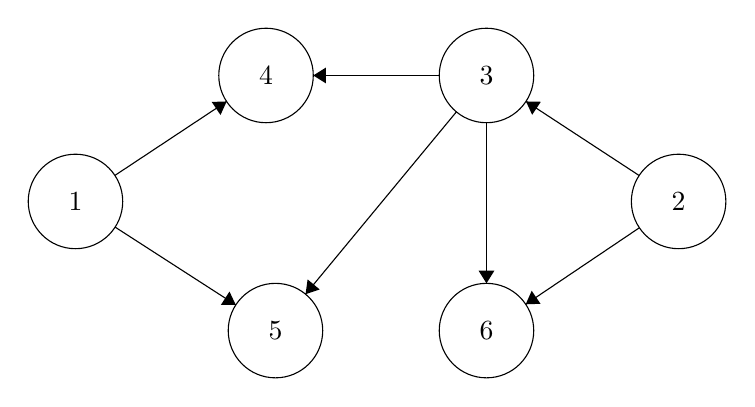
\begin{tikzpicture}[scale=0.2]
		\tikzstyle{every node}+=[inner sep=0pt]
		\draw [black] (13,-24.1) circle (3);
		\draw (13,-24.1) node {$1$};
		\draw [black] (51.3,-24.1) circle (3);
		\draw (51.3,-24.1) node {$2$};
		\draw [black] (39.1,-16.1) circle (3);
		\draw (39.1,-16.1) node {$3$};
		\draw [black] (25.1,-16.1) circle (3);
		\draw (25.1,-16.1) node {$4$};
		\draw [black] (25.7,-32.3) circle (3);
		\draw (25.7,-32.3) node {$5$};
		\draw [black] (39.1,-32.3) circle (3);
		\draw (39.1,-32.3) node {$6$};
		\draw [black] (15.5,-22.45) -- (22.6,-17.75);
		\fill [black] (22.6,-17.75) -- (21.65,-17.78) -- (22.21,-18.61);
		\draw [black] (15.52,-25.73) -- (23.18,-30.67);
		\fill [black] (23.18,-30.67) -- (22.78,-29.82) -- (22.24,-30.66);
		\draw [black] (48.79,-22.45) -- (41.61,-17.75);
		\fill [black] (41.61,-17.75) -- (42,-18.6) -- (42.55,-17.77);
		\draw [black] (48.81,-25.77) -- (41.59,-30.63);
		\fill [black] (41.59,-30.63) -- (42.53,-30.6) -- (41.97,-29.77);
		\draw [black] (36.1,-16.1) -- (28.1,-16.1);
		\fill [black] (28.1,-16.1) -- (28.9,-16.6) -- (28.9,-15.6);
		\draw [black] (37.19,-18.41) -- (27.61,-29.99);
		\fill [black] (27.61,-29.99) -- (28.51,-29.69) -- (27.74,-29.05);
		\draw [black] (39.1,-19.1) -- (39.1,-29.3);
		\fill [black] (39.1,-29.3) -- (39.6,-28.5) -- (38.6,-28.5);
	\end{tikzpicture}
\caption{Non-optimal Hill-Climbing Influence Diagram}
\label{diagram:non_optimal_hill_climbing}
\end{figure}

Then note that greedy hill climbing will start with $S_0 = \emptyset$ and then proceed to choose node $3$ (as it has the highest influence), so that $S_1 = \{3\}$ and $f(S_1) = 4$. For the next step, note that nodes $4,5,6$ only influece themselves, so the marginal influence is $0$, and that both nodes $1$ and $2$ influece nodes already influenced by $3$, so their marginal influece is both $1$. Therefore the algorithm will chose at random either $1$ or $2$. Let us suppose $2$, then we have $S_2 = \{2,3\}$ with $f(S_2) = 4$.

However, note that the optimal set is $T = \{1,2\}$ for which we have $f(T) = 6$.

% Question 4.2
\newquestion{4.2}
For $i = 3$, construct an example where f(Si) ≤ 0.8f(T). That is, hill-climbing will only find a
solution that is at most 80% of the optimal solution.

% Question 4.3
\newquestion{4.3}

% Question 4.4
\newquestion{4.4}

% Information sheet
% Fill out the information below (this should be the last page of your assignment)
\addinformationsheet
{\Large
\textbf{Your name:} Luis Perez  % Put your name here
\\
\textbf{Email:} luis0@stanford.edu \hspace*{7cm}  % Put your e-mail here
\textbf{SUID:} 05794739  % Put your student ID here
\\*[2ex] 
}
Discussion Group: None   % List your study group here
\\
\vfill\vfill
I acknowledge and accept the Honor Code.\\*[3ex]
\bigskip
\textit{(Signed)} 
LAP
\vfill





\end{document}